\documentclass[10pt,a4paper]{article}

\usepackage[margin=2.0cm]{geometry}
\usepackage{amsmath,amssymb}
\usepackage{graphicx}
\usepackage{booktabs}
\usepackage{array}
\usepackage{tabularx}
\usepackage{longtable}
\usepackage{multirow}
\usepackage{threeparttable}
\usepackage{xcolor}
\usepackage{caption}
\usepackage{subcaption}
\usepackage{float}
\usepackage{xurl}
\usepackage{hyperref}
\usepackage{microtype}

\graphicspath{{../figures/}{../figures/supplementary/}}
\hypersetup{colorlinks=true,linkcolor=blue!55!black,citecolor=blue!55!black,urlcolor=blue!55!black}
\setlength{\parindent}{0pt}
\setlength{\parskip}{4pt}
\setlength{\emergencystretch}{3em}
\captionsetup{font=small,labelfont=bf}
\newcolumntype{Y}{>{\raggedright\arraybackslash}X}
\renewcommand{\thetable}{S\arabic{table}}
\renewcommand{\thefigure}{S\arabic{figure}}

\begin{document}

\begin{center}
{\Large\bfseries Supplementary Information\par}
\vspace{0.5cm}
{\large An Accuracy and Calibration Benchmark of scGPT Pipelines and Matched Classical Models for Cell Type Annotation\par}
\vspace{0.4cm}
{\normalsize Alireza Khosravi et al.\par}
\end{center}

\section*{Contents}
This file reports the complete outer-fold results, pooled out-of-fold metrics, paired donor-cluster bootstrap comparisons, hyperparameter selections, calibration sensitivity, strict label-scarcity analysis, per-class error analysis, and the separately designated pig-pancreas cross-species stress test. The machine-readable source tables and prediction-level audit files are included in the accompanying reproducibility archive.

\section{Completed human benchmark}

\begin{table}[H]
\centering
\caption{Completed out-of-fold design audit.}
\label{tab:design-audit}
\small
\begin{tabular}{lrrrr}
\toprule
Dataset & Donor IDs & Classes & OOF cells & Matched HVGs \\
\midrule
TNBC & 101 & 7 & 427,813 & 1167--1172 \\
PBMC & 199 & 13 & 462,034 & 1132--1141 \\
Brain & 12 & 10 & 75,580 & 930--953 \\
\bottomrule
\end{tabular}
\end{table}


\begin{figure}[H]\centering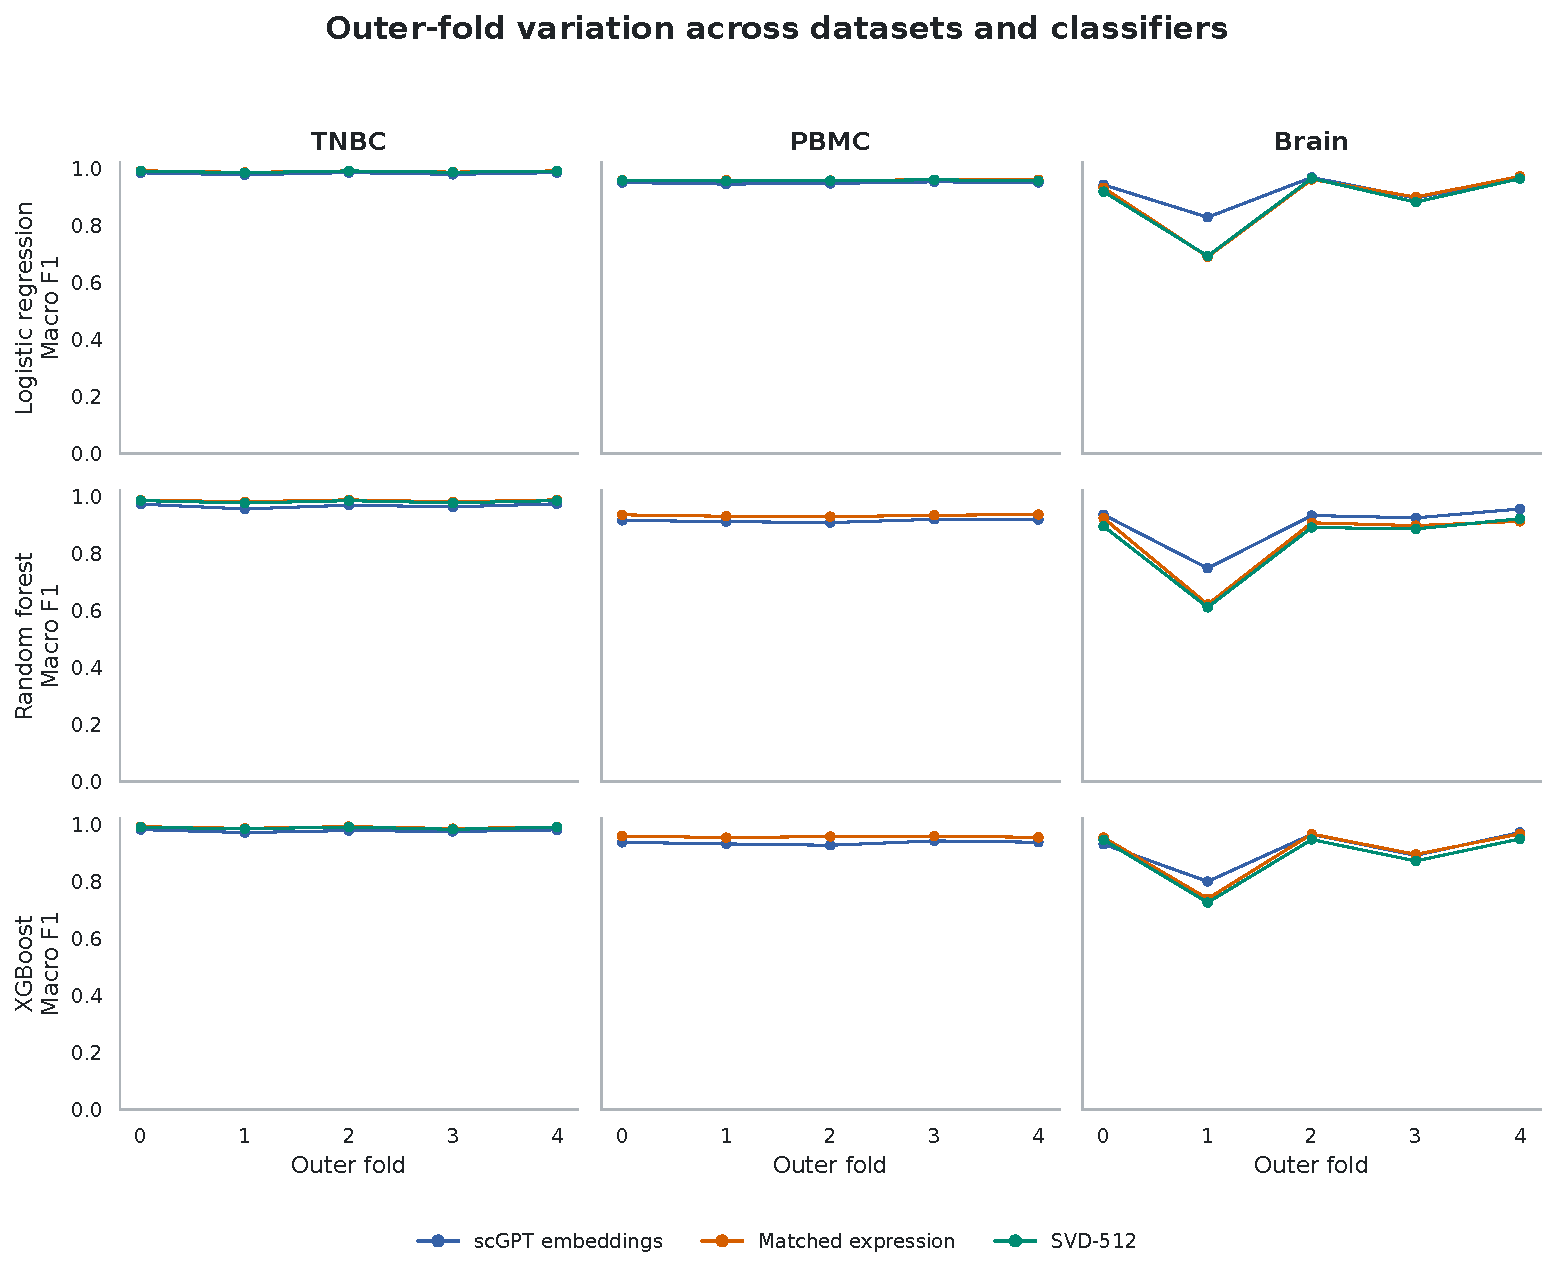
\includegraphics[width=\textwidth]{supplementary_outer_fold_variation.pdf}\caption{Outer-fold Macro F1 for every human representation--classifier pipeline. Training folds overlap, but each outer-test donor and cell occurs in exactly one fold.}\label{fig:s-folds}\end{figure}

\clearpage\section{Five-fold pipeline coverage}

{\footnotesize\setlength{\tabcolsep}{3pt}
\begin{longtable}{llll}
\caption{Pipeline coverage used by the local aggregation. A pipeline was included only when all five aligned donor-held-out prediction folds were durably available.}\label{tab:s-coverage}\\
\toprule
Dataset & Representation & Classifier & Status \\
\midrule
\endfirsthead
\multicolumn{4}{c}{\tablename\ \thetable{} continued}\\
\toprule
Dataset & Representation & Classifier & Status \\
\midrule
\endhead
\midrule
\multicolumn{4}{r}{Continued on next page}\\
\endfoot
\bottomrule
\endlastfoot
Brain & Matched expression & Logistic regression & Included \\
Brain & Matched expression & Random forest & Included \\
Brain & Matched expression & XGBoost & Included \\
Brain & scGPT embeddings & Logistic regression & Included \\
Brain & scGPT embeddings & Random forest & Included \\
Brain & scGPT embeddings & XGBoost & Included \\
Brain & SVD-512 & Logistic regression & Included \\
Brain & SVD-512 & Random forest & Included \\
Brain & SVD-512 & XGBoost & Included \\
PBMC & Matched expression & Logistic regression & Included \\
PBMC & Matched expression & Random forest & Included \\
PBMC & Matched expression & XGBoost & Included \\
PBMC & scGPT embeddings & Logistic regression & Included \\
PBMC & scGPT embeddings & Random forest & Included \\
PBMC & scGPT embeddings & XGBoost & Included \\
PBMC & SVD-512 & Logistic regression & Included \\
PBMC & SVD-512 & Random forest & Not available \\
PBMC & SVD-512 & XGBoost & Not available \\
TNBC & Matched expression & Logistic regression & Included \\
TNBC & Matched expression & Random forest & Included \\
TNBC & Matched expression & XGBoost & Included \\
TNBC & scGPT embeddings & Logistic regression & Included \\
TNBC & scGPT embeddings & Random forest & Included \\
TNBC & scGPT embeddings & XGBoost & Included \\
TNBC & SVD-512 & Logistic regression & Included \\
TNBC & SVD-512 & Random forest & Included \\
TNBC & SVD-512 & XGBoost & Included \\
\end{longtable}
}

\clearpage\section{Pooled out-of-fold metrics}

{\footnotesize\setlength{\tabcolsep}{3pt}
\begin{longtable}{lllrrrrrrr}
\caption{Complete pooled out-of-fold metrics for the three human atlases. SVD-512 cells are blank in the main table where a five-fold classifier pipeline was not available.}\label{tab:s-pooled}\\
\toprule
Dataset & Representation & Classifier & $n$ & Macro F1 & Accuracy & Balanced acc. & ECE & Brier & NLL \\
\midrule
\endfirsthead
\multicolumn{10}{c}{\tablename\ \thetable{} continued}\\
\toprule
Dataset & Representation & Classifier & $n$ & Macro F1 & Accuracy & Balanced acc. & ECE & Brier & NLL \\
\midrule
\endhead
\midrule
\multicolumn{10}{r}{Continued on next page}\\
\endfoot
\bottomrule
\endlastfoot
Brain & Matched expression & Logistic regression & 75580 & 0.911 & 0.985 & 0.874 & 0.004 & 0.027 & 0.107 \\
Brain & scGPT embeddings & Logistic regression & 75580 & 0.940 & 0.986 & 0.915 & 0.003 & 0.025 & 0.070 \\
Brain & SVD-512 & Logistic regression & 75580 & 0.906 & 0.985 & 0.872 & 0.004 & 0.027 & 0.106 \\
Brain & Matched expression & Random forest & 75580 & 0.870 & 0.983 & 0.807 & 0.021 & 0.032 & 0.156 \\
Brain & scGPT embeddings & Random forest & 75580 & 0.908 & 0.984 & 0.859 & 0.020 & 0.032 & 0.132 \\
Brain & SVD-512 & Random forest & 75580 & 0.848 & 0.985 & 0.790 & 0.011 & 0.028 & 0.160 \\
Brain & Matched expression & XGBoost & 75580 & 0.925 & 0.987 & 0.887 & 0.008 & 0.024 & 0.072 \\
Brain & scGPT embeddings & XGBoost & 75580 & 0.930 & 0.986 & 0.903 & 0.009 & 0.026 & 0.081 \\
Brain & SVD-512 & XGBoost & 75580 & 0.904 & 0.987 & 0.856 & 0.010 & 0.024 & 0.092 \\
PBMC & Matched expression & Logistic regression & 462034 & 0.959 & 0.953 & 0.957 & 0.004 & 0.069 & 0.121 \\
PBMC & scGPT embeddings & Logistic regression & 462034 & 0.949 & 0.940 & 0.947 & 0.002 & 0.089 & 0.159 \\
PBMC & SVD-512 & Logistic regression & 462034 & 0.958 & 0.952 & 0.955 & 0.003 & 0.071 & 0.125 \\
PBMC & Matched expression & Random forest & 462034 & 0.933 & 0.941 & 0.914 & 0.039 & 0.094 & 0.186 \\
PBMC & scGPT embeddings & Random forest & 462034 & 0.915 & 0.907 & 0.897 & 0.059 & 0.148 & 0.281 \\
PBMC & Matched expression & XGBoost & 462034 & 0.957 & 0.953 & 0.953 & 0.003 & 0.070 & 0.123 \\
PBMC & scGPT embeddings & XGBoost & 462034 & 0.935 & 0.925 & 0.929 & 0.004 & 0.111 & 0.199 \\
TNBC & Matched expression & Logistic regression & 427813 & 0.990 & 0.988 & 0.988 & 0.000 & 0.019 & 0.038 \\
TNBC & scGPT embeddings & Logistic regression & 427813 & 0.983 & 0.979 & 0.981 & 0.001 & 0.033 & 0.065 \\
TNBC & SVD-512 & Logistic regression & 427813 & 0.989 & 0.987 & 0.988 & 0.001 & 0.020 & 0.040 \\
TNBC & Matched expression & Random forest & 427813 & 0.985 & 0.984 & 0.978 & 0.037 & 0.031 & 0.078 \\
TNBC & scGPT embeddings & Random forest & 427813 & 0.968 & 0.964 & 0.953 & 0.038 & 0.061 & 0.134 \\
TNBC & SVD-512 & Random forest & 427813 & 0.982 & 0.979 & 0.977 & 0.023 & 0.037 & 0.081 \\
TNBC & Matched expression & XGBoost & 427813 & 0.990 & 0.989 & 0.987 & 0.001 & 0.018 & 0.035 \\
TNBC & scGPT embeddings & XGBoost & 427813 & 0.978 & 0.974 & 0.972 & 0.001 & 0.040 & 0.077 \\
TNBC & SVD-512 & XGBoost & 427813 & 0.988 & 0.986 & 0.986 & 0.003 & 0.022 & 0.043 \\
\end{longtable}
}

\clearpage\section{Outer-fold metrics}

{\footnotesize\setlength{\tabcolsep}{3pt}
\begin{longtable}{lrllrrrrrr}
\caption{Outer-fold metrics. Fold-level values are not independent because their training partitions overlap.}\label{tab:s-fold}\\
\toprule
Dataset & Fold & Representation & Classifier & Groups & Cells & Macro F1 & Accuracy & ECE & Brier \\
\midrule
\endfirsthead
\multicolumn{10}{c}{\tablename\ \thetable{} continued}\\
\toprule
Dataset & Fold & Representation & Classifier & Groups & Cells & Macro F1 & Accuracy & ECE & Brier \\
\midrule
\endhead
\midrule
\multicolumn{10}{r}{Continued on next page}\\
\endfoot
\bottomrule
\endlastfoot
Brain & 0 & Matched expression & Logistic regression & 3 & 19314 & 0.932 & 0.973 & 0.024 & 0.051 \\
Brain & 1 & Matched expression & Logistic regression & 1 & 11034 & 0.690 & 0.966 & 0.008 & 0.053 \\
Brain & 2 & Matched expression & Logistic regression & 3 & 15401 & 0.961 & 0.994 & 0.005 & 0.011 \\
Brain & 3 & Matched expression & Logistic regression & 3 & 14244 & 0.900 & 0.994 & 0.006 & 0.012 \\
Brain & 4 & Matched expression & Logistic regression & 2 & 15587 & 0.972 & 0.996 & 0.013 & 0.008 \\
Brain & 0 & scGPT embeddings & Logistic regression & 3 & 19314 & 0.943 & 0.978 & 0.015 & 0.043 \\
Brain & 1 & scGPT embeddings & Logistic regression & 1 & 11034 & 0.829 & 0.973 & 0.012 & 0.045 \\
Brain & 2 & scGPT embeddings & Logistic regression & 3 & 15401 & 0.969 & 0.994 & 0.008 & 0.010 \\
Brain & 3 & scGPT embeddings & Logistic regression & 3 & 14244 & 0.896 & 0.992 & 0.012 & 0.016 \\
Brain & 4 & scGPT embeddings & Logistic regression & 2 & 15587 & 0.968 & 0.994 & 0.006 & 0.010 \\
Brain & 0 & SVD-512 & Logistic regression & 3 & 19314 & 0.919 & 0.973 & 0.023 & 0.051 \\
Brain & 1 & SVD-512 & Logistic regression & 1 & 11034 & 0.693 & 0.966 & 0.008 & 0.052 \\
Brain & 2 & SVD-512 & Logistic regression & 3 & 15401 & 0.965 & 0.994 & 0.005 & 0.010 \\
Brain & 3 & SVD-512 & Logistic regression & 3 & 14244 & 0.882 & 0.993 & 0.001 & 0.012 \\
Brain & 4 & SVD-512 & Logistic regression & 2 & 15587 & 0.964 & 0.995 & 0.018 & 0.009 \\
Brain & 0 & Matched expression & Random forest & 3 & 19314 & 0.924 & 0.977 & 0.013 & 0.045 \\
Brain & 1 & Matched expression & Random forest & 1 & 11034 & 0.621 & 0.960 & 0.021 & 0.067 \\
Brain & 2 & Matched expression & Random forest & 3 & 15401 & 0.908 & 0.990 & 0.027 & 0.018 \\
Brain & 3 & Matched expression & Random forest & 3 & 14244 & 0.898 & 0.991 & 0.023 & 0.020 \\
Brain & 4 & Matched expression & Random forest & 2 & 15587 & 0.913 & 0.994 & 0.033 & 0.016 \\
Brain & 0 & scGPT embeddings & Random forest & 3 & 19314 & 0.936 & 0.977 & 0.016 & 0.046 \\
Brain & 1 & scGPT embeddings & Random forest & 1 & 11034 & 0.748 & 0.966 & 0.008 & 0.057 \\
Brain & 2 & scGPT embeddings & Random forest & 3 & 15401 & 0.933 & 0.990 & 0.036 & 0.021 \\
Brain & 3 & scGPT embeddings & Random forest & 3 & 14244 & 0.925 & 0.992 & 0.030 & 0.021 \\
Brain & 4 & scGPT embeddings & Random forest & 2 & 15587 & 0.956 & 0.993 & 0.025 & 0.016 \\
Brain & 0 & SVD-512 & Random forest & 3 & 19314 & 0.895 & 0.978 & 0.018 & 0.045 \\
Brain & 1 & SVD-512 & Random forest & 1 & 11034 & 0.611 & 0.964 & 0.003 & 0.055 \\
Brain & 2 & SVD-512 & Random forest & 3 & 15401 & 0.891 & 0.993 & 0.020 & 0.015 \\
Brain & 3 & SVD-512 & Random forest & 3 & 14244 & 0.886 & 0.993 & 0.017 & 0.015 \\
Brain & 4 & SVD-512 & Random forest & 2 & 15587 & 0.922 & 0.995 & 0.021 & 0.013 \\
Brain & 0 & Matched expression & XGBoost & 3 & 19314 & 0.954 & 0.979 & 0.019 & 0.041 \\
Brain & 1 & Matched expression & XGBoost & 1 & 11034 & 0.739 & 0.970 & 0.020 & 0.051 \\
Brain & 2 & Matched expression & XGBoost & 3 & 15401 & 0.966 & 0.995 & 0.004 & 0.009 \\
Brain & 3 & Matched expression & XGBoost & 3 & 14244 & 0.895 & 0.992 & 0.003 & 0.014 \\
Brain & 4 & Matched expression & XGBoost & 2 & 15587 & 0.967 & 0.995 & 0.001 & 0.008 \\
Brain & 0 & scGPT embeddings & XGBoost & 3 & 19314 & 0.931 & 0.977 & 0.019 & 0.043 \\
Brain & 1 & scGPT embeddings & XGBoost & 1 & 11034 & 0.800 & 0.971 & 0.025 & 0.053 \\
Brain & 2 & scGPT embeddings & XGBoost & 3 & 15401 & 0.965 & 0.994 & 0.003 & 0.011 \\
Brain & 3 & scGPT embeddings & XGBoost & 3 & 14244 & 0.891 & 0.992 & 0.002 & 0.015 \\
Brain & 4 & scGPT embeddings & XGBoost & 2 & 15587 & 0.972 & 0.994 & 0.003 & 0.009 \\
Brain & 0 & SVD-512 & XGBoost & 3 & 19314 & 0.946 & 0.978 & 0.020 & 0.042 \\
Brain & 1 & SVD-512 & XGBoost & 1 & 11034 & 0.726 & 0.971 & 0.024 & 0.053 \\
Brain & 2 & SVD-512 & XGBoost & 3 & 15401 & 0.947 & 0.994 & 0.003 & 0.010 \\
Brain & 3 & SVD-512 & XGBoost & 3 & 14244 & 0.872 & 0.993 & 0.005 & 0.012 \\
Brain & 4 & SVD-512 & XGBoost & 2 & 15587 & 0.949 & 0.995 & 0.002 & 0.008 \\
PBMC & 0 & Matched expression & Logistic regression & 40 & 93930 & 0.959 & 0.953 & 0.005 & 0.070 \\
PBMC & 1 & Matched expression & Logistic regression & 38 & 92275 & 0.959 & 0.952 & 0.002 & 0.071 \\
PBMC & 2 & Matched expression & Logistic regression & 42 & 93316 & 0.958 & 0.952 & 0.004 & 0.071 \\
PBMC & 3 & Matched expression & Logistic regression & 38 & 90015 & 0.960 & 0.955 & 0.004 & 0.066 \\
PBMC & 4 & Matched expression & Logistic regression & 41 & 92498 & 0.960 & 0.955 & 0.004 & 0.066 \\
PBMC & 0 & scGPT embeddings & Logistic regression & 40 & 93930 & 0.951 & 0.940 & 0.003 & 0.090 \\
PBMC & 1 & scGPT embeddings & Logistic regression & 38 & 92275 & 0.945 & 0.937 & 0.003 & 0.093 \\
PBMC & 2 & scGPT embeddings & Logistic regression & 42 & 93316 & 0.948 & 0.938 & 0.002 & 0.093 \\
PBMC & 3 & scGPT embeddings & Logistic regression & 38 & 90015 & 0.953 & 0.944 & 0.001 & 0.085 \\
PBMC & 4 & scGPT embeddings & Logistic regression & 41 & 92498 & 0.951 & 0.943 & 0.002 & 0.085 \\
PBMC & 0 & SVD-512 & Logistic regression & 40 & 93930 & 0.958 & 0.951 & 0.003 & 0.072 \\
PBMC & 1 & SVD-512 & Logistic regression & 38 & 92275 & 0.956 & 0.949 & 0.002 & 0.074 \\
PBMC & 2 & SVD-512 & Logistic regression & 42 & 93316 & 0.957 & 0.951 & 0.002 & 0.072 \\
PBMC & 3 & SVD-512 & Logistic regression & 38 & 90015 & 0.960 & 0.955 & 0.002 & 0.068 \\
PBMC & 4 & SVD-512 & Logistic regression & 41 & 92498 & 0.956 & 0.953 & 0.006 & 0.069 \\
PBMC & 0 & Matched expression & Random forest & 40 & 93930 & 0.935 & 0.941 & 0.037 & 0.094 \\
PBMC & 1 & Matched expression & Random forest & 38 & 92275 & 0.931 & 0.937 & 0.040 & 0.099 \\
PBMC & 2 & Matched expression & Random forest & 42 & 93316 & 0.929 & 0.939 & 0.041 & 0.097 \\
PBMC & 3 & Matched expression & Random forest & 38 & 90015 & 0.934 & 0.944 & 0.039 & 0.090 \\
PBMC & 4 & Matched expression & Random forest & 41 & 92498 & 0.937 & 0.944 & 0.037 & 0.089 \\
PBMC & 0 & scGPT embeddings & Random forest & 40 & 93930 & 0.916 & 0.907 & 0.059 & 0.149 \\
PBMC & 1 & scGPT embeddings & Random forest & 38 & 92275 & 0.912 & 0.904 & 0.057 & 0.151 \\
PBMC & 2 & scGPT embeddings & Random forest & 42 & 93316 & 0.908 & 0.901 & 0.064 & 0.159 \\
PBMC & 3 & scGPT embeddings & Random forest & 38 & 90015 & 0.920 & 0.912 & 0.056 & 0.141 \\
PBMC & 4 & scGPT embeddings & Random forest & 41 & 92498 & 0.919 & 0.912 & 0.057 & 0.141 \\
PBMC & 0 & Matched expression & XGBoost & 40 & 93930 & 0.960 & 0.953 & 0.004 & 0.069 \\
PBMC & 1 & Matched expression & XGBoost & 38 & 92275 & 0.954 & 0.950 & 0.005 & 0.073 \\
PBMC & 2 & Matched expression & XGBoost & 42 & 93316 & 0.958 & 0.953 & 0.002 & 0.070 \\
PBMC & 3 & Matched expression & XGBoost & 38 & 90015 & 0.959 & 0.956 & 0.003 & 0.065 \\
PBMC & 4 & Matched expression & XGBoost & 41 & 92498 & 0.955 & 0.952 & 0.007 & 0.071 \\
PBMC & 0 & scGPT embeddings & XGBoost & 40 & 93930 & 0.937 & 0.927 & 0.008 & 0.109 \\
PBMC & 1 & scGPT embeddings & XGBoost & 38 & 92275 & 0.932 & 0.923 & 0.010 & 0.114 \\
PBMC & 2 & scGPT embeddings & XGBoost & 42 & 93316 & 0.927 & 0.916 & 0.006 & 0.124 \\
PBMC & 3 & scGPT embeddings & XGBoost & 38 & 90015 & 0.942 & 0.930 & 0.003 & 0.103 \\
PBMC & 4 & scGPT embeddings & XGBoost & 41 & 92498 & 0.937 & 0.930 & 0.007 & 0.104 \\
TNBC & 0 & Matched expression & Logistic regression & 19 & 85988 & 0.992 & 0.990 & 0.001 & 0.015 \\
TNBC & 1 & Matched expression & Logistic regression & 20 & 84601 & 0.986 & 0.984 & 0.003 & 0.025 \\
TNBC & 2 & Matched expression & Logistic regression & 21 & 86821 & 0.991 & 0.990 & 0.006 & 0.016 \\
TNBC & 3 & Matched expression & Logistic regression & 21 & 86079 & 0.987 & 0.985 & 0.002 & 0.024 \\
TNBC & 4 & Matched expression & Logistic regression & 20 & 84324 & 0.991 & 0.989 & 0.001 & 0.017 \\
TNBC & 0 & scGPT embeddings & Logistic regression & 19 & 85988 & 0.985 & 0.982 & 0.004 & 0.028 \\
TNBC & 1 & scGPT embeddings & Logistic regression & 20 & 84601 & 0.978 & 0.972 & 0.003 & 0.042 \\
TNBC & 2 & scGPT embeddings & Logistic regression & 21 & 86821 & 0.985 & 0.982 & 0.001 & 0.028 \\
TNBC & 3 & scGPT embeddings & Logistic regression & 21 & 86079 & 0.979 & 0.976 & 0.005 & 0.037 \\
TNBC & 4 & scGPT embeddings & Logistic regression & 20 & 84324 & 0.985 & 0.981 & 0.001 & 0.029 \\
TNBC & 0 & SVD-512 & Logistic regression & 19 & 85988 & 0.991 & 0.989 & 0.001 & 0.016 \\
TNBC & 1 & SVD-512 & Logistic regression & 20 & 84601 & 0.985 & 0.983 & 0.003 & 0.027 \\
TNBC & 2 & SVD-512 & Logistic regression & 21 & 86821 & 0.991 & 0.989 & 0.001 & 0.017 \\
TNBC & 3 & SVD-512 & Logistic regression & 21 & 86079 & 0.987 & 0.984 & 0.002 & 0.025 \\
TNBC & 4 & SVD-512 & Logistic regression & 20 & 84324 & 0.991 & 0.989 & 0.001 & 0.018 \\
TNBC & 0 & Matched expression & Random forest & 19 & 85988 & 0.987 & 0.986 & 0.037 & 0.027 \\
TNBC & 1 & Matched expression & Random forest & 20 & 84601 & 0.981 & 0.982 & 0.037 & 0.034 \\
TNBC & 2 & Matched expression & Random forest & 21 & 86821 & 0.988 & 0.988 & 0.039 & 0.027 \\
TNBC & 3 & Matched expression & Random forest & 21 & 86079 & 0.981 & 0.979 & 0.036 & 0.040 \\
TNBC & 4 & Matched expression & Random forest & 20 & 84324 & 0.988 & 0.987 & 0.038 & 0.027 \\
TNBC & 0 & scGPT embeddings & Random forest & 19 & 85988 & 0.973 & 0.970 & 0.043 & 0.053 \\
TNBC & 1 & scGPT embeddings & Random forest & 20 & 84601 & 0.956 & 0.957 & 0.038 & 0.072 \\
TNBC & 2 & scGPT embeddings & Random forest & 21 & 86821 & 0.969 & 0.964 & 0.035 & 0.059 \\
TNBC & 3 & scGPT embeddings & Random forest & 21 & 86079 & 0.963 & 0.959 & 0.029 & 0.066 \\
TNBC & 4 & scGPT embeddings & Random forest & 20 & 84324 & 0.974 & 0.971 & 0.044 & 0.052 \\
TNBC & 0 & SVD-512 & Random forest & 19 & 85988 & 0.985 & 0.982 & 0.025 & 0.032 \\
TNBC & 1 & SVD-512 & Random forest & 20 & 84601 & 0.977 & 0.973 & 0.021 & 0.045 \\
TNBC & 2 & SVD-512 & Random forest & 21 & 86821 & 0.985 & 0.982 & 0.029 & 0.035 \\
TNBC & 3 & SVD-512 & Random forest & 21 & 86079 & 0.978 & 0.974 & 0.018 & 0.042 \\
TNBC & 4 & SVD-512 & Random forest & 20 & 84324 & 0.985 & 0.983 & 0.023 & 0.030 \\
TNBC & 0 & Matched expression & XGBoost & 19 & 85988 & 0.992 & 0.991 & 0.002 & 0.014 \\
TNBC & 1 & Matched expression & XGBoost & 20 & 84601 & 0.986 & 0.986 & 0.001 & 0.021 \\
TNBC & 2 & Matched expression & XGBoost & 21 & 86821 & 0.993 & 0.992 & 0.002 & 0.013 \\
TNBC & 3 & Matched expression & XGBoost & 21 & 86079 & 0.985 & 0.984 & 0.003 & 0.024 \\
TNBC & 4 & Matched expression & XGBoost & 20 & 84324 & 0.991 & 0.990 & 0.005 & 0.016 \\
TNBC & 0 & scGPT embeddings & XGBoost & 19 & 85988 & 0.982 & 0.980 & 0.001 & 0.031 \\
TNBC & 1 & scGPT embeddings & XGBoost & 20 & 84601 & 0.971 & 0.968 & 0.006 & 0.048 \\
TNBC & 2 & scGPT embeddings & XGBoost & 21 & 86821 & 0.979 & 0.975 & 0.004 & 0.039 \\
TNBC & 3 & scGPT embeddings & XGBoost & 21 & 86079 & 0.975 & 0.971 & 0.010 & 0.045 \\
TNBC & 4 & scGPT embeddings & XGBoost & 20 & 84324 & 0.981 & 0.976 & 0.005 & 0.036 \\
TNBC & 0 & SVD-512 & XGBoost & 19 & 85988 & 0.990 & 0.988 & 0.005 & 0.018 \\
TNBC & 1 & SVD-512 & XGBoost & 20 & 84601 & 0.985 & 0.982 & 0.003 & 0.028 \\
TNBC & 2 & SVD-512 & XGBoost & 21 & 86821 & 0.991 & 0.990 & 0.000 & 0.016 \\
TNBC & 3 & SVD-512 & XGBoost & 21 & 86079 & 0.983 & 0.981 & 0.002 & 0.029 \\
TNBC & 4 & SVD-512 & XGBoost & 20 & 84324 & 0.990 & 0.988 & 0.006 & 0.019 \\
\end{longtable}
}

\clearpage\section{SVD-512 dimensionality control}

{\footnotesize\setlength{\tabcolsep}{3pt}
\begin{longtable}{lrrrrr}
\caption{Fold-specific SVD-512 audit. Decomposition parameters were fitted without outer-test cells.}\label{tab:s-svd}\\
\toprule
Dataset & Fold & Components & Fit cells & Explained variance & Training only \\
\midrule
\endfirsthead
\multicolumn{6}{c}{\tablename\ \thetable{} continued}\\
\toprule
Dataset & Fold & Components & Fit cells & Explained variance & Training only \\
\midrule
\endhead
\midrule
\multicolumn{6}{r}{Continued on next page}\\
\endfoot
\bottomrule
\endlastfoot
Brain & 0 & 512 & 56,266 & 0.935 & Yes \\
Brain & 1 & 512 & 64,547 & 0.939 & Yes \\
Brain & 2 & 512 & 60,179 & 0.942 & Yes \\
Brain & 3 & 512 & 61,336 & 0.939 & Yes \\
Brain & 4 & 512 & 59,996 & 0.934 & Yes \\
PBMC & 0 & 512 & 100,000 & 0.959 & Yes \\
PBMC & 1 & 512 & 100,000 & 0.958 & Yes \\
PBMC & 2 & 512 & 100,000 & 0.958 & Yes \\
PBMC & 3 & 512 & 100,000 & 0.959 & Yes \\
PBMC & 4 & 512 & 100,000 & 0.959 & Yes \\
TNBC & 0 & 512 & 100,000 & 0.954 & Yes \\
TNBC & 1 & 512 & 100,000 & 0.954 & Yes \\
TNBC & 2 & 512 & 100,000 & 0.954 & Yes \\
TNBC & 3 & 512 & 100,000 & 0.956 & Yes \\
TNBC & 4 & 512 & 100,000 & 0.955 & Yes \\
\end{longtable}
}

\clearpage\section{Donor-cluster bootstrap comparisons}

{\footnotesize\setlength{\tabcolsep}{3pt}
\begin{longtable}{lllrrrrr}
\caption{All paired donor-cluster bootstrap contrasts. Intervals condition on the fitted pipelines.}\label{tab:s-bootstrap}\\
\toprule
Dataset & Classifier & Contrast & A & B & $A-B$ & 95\% interval & $P(A>B)$ \\
\midrule
\endfirsthead
\multicolumn{8}{c}{\tablename\ \thetable{} continued}\\
\toprule
Dataset & Classifier & Contrast & A & B & $A-B$ & 95\% interval & $P(A>B)$ \\
\midrule
\endhead
\midrule
\multicolumn{8}{r}{Continued on next page}\\
\endfoot
\bottomrule
\endlastfoot
Brain & Logistic regression & Expression $-$ scGPT & 0.911 & 0.940 & -0.028 & [-0.072, 0.004] & 0.081 \\
Brain & Random forest & Expression $-$ scGPT & 0.870 & 0.908 & -0.039 & [-0.066, -0.014] & 0.000 \\
Brain & XGBoost & Expression $-$ scGPT & 0.925 & 0.930 & -0.005 & [-0.024, 0.014] & 0.334 \\
PBMC & Logistic regression & Expression $-$ scGPT & 0.959 & 0.949 & 0.010 & [0.009, 0.011] & 1.000 \\
PBMC & Random forest & Expression $-$ scGPT & 0.933 & 0.915 & 0.018 & [0.016, 0.020] & 1.000 \\
PBMC & XGBoost & Expression $-$ scGPT & 0.957 & 0.935 & 0.022 & [0.020, 0.024] & 1.000 \\
TNBC & Logistic regression & Expression $-$ scGPT & 0.990 & 0.983 & 0.007 & [0.006, 0.008] & 1.000 \\
TNBC & Random forest & Expression $-$ scGPT & 0.985 & 0.968 & 0.018 & [0.014, 0.022] & 1.000 \\
TNBC & XGBoost & Expression $-$ scGPT & 0.990 & 0.978 & 0.012 & [0.010, 0.014] & 1.000 \\
Brain & Logistic regression & Expression $-$ SVD & 0.911 & 0.906 & 0.005 & [-0.001, 0.012] & 0.950 \\
Brain & Random forest & Expression $-$ SVD & 0.870 & 0.848 & 0.022 & [0.009, 0.035] & 1.000 \\
Brain & XGBoost & Expression $-$ SVD & 0.925 & 0.904 & 0.021 & [0.013, 0.030] & 1.000 \\
PBMC & Logistic regression & Expression $-$ SVD & 0.959 & 0.958 & 0.002 & [0.001, 0.003] & 1.000 \\
TNBC & Logistic regression & Expression $-$ SVD & 0.990 & 0.989 & 0.001 & [0.000, 0.001] & 1.000 \\
TNBC & Random forest & Expression $-$ SVD & 0.985 & 0.982 & 0.003 & [0.002, 0.005] & 1.000 \\
TNBC & XGBoost & Expression $-$ SVD & 0.990 & 0.988 & 0.002 & [0.001, 0.003] & 0.998 \\
Brain & Logistic regression & SVD $-$ scGPT & 0.906 & 0.940 & -0.033 & [-0.075, -0.003] & 0.003 \\
Brain & Random forest & SVD $-$ scGPT & 0.848 & 0.908 & -0.060 & [-0.096, -0.030] & 0.000 \\
Brain & XGBoost & SVD $-$ scGPT & 0.904 & 0.930 & -0.026 & [-0.048, -0.002] & 0.016 \\
PBMC & Logistic regression & SVD $-$ scGPT & 0.958 & 0.949 & 0.008 & [0.007, 0.009] & 1.000 \\
TNBC & Logistic regression & SVD $-$ scGPT & 0.989 & 0.983 & 0.007 & [0.005, 0.008] & 1.000 \\
TNBC & Random forest & SVD $-$ scGPT & 0.982 & 0.968 & 0.015 & [0.012, 0.018] & 1.000 \\
TNBC & XGBoost & SVD $-$ scGPT & 0.988 & 0.978 & 0.010 & [0.009, 0.012] & 1.000 \\
\end{longtable}
}

\clearpage\section{Training-only model selection}

{\footnotesize\setlength{\tabcolsep}{3pt}
\begin{longtable}{lll>{\raggedright\arraybackslash}p{6.8cm}r}
\caption{Frequencies of independently selected parameter sets across the five outer folds.}\label{tab:s-parameters}\\
\toprule
Dataset & Representation & Classifier & Selected parameter set & Folds \\
\midrule
\endfirsthead
\multicolumn{5}{c}{\tablename\ \thetable{} continued}\\
\toprule
Dataset & Representation & Classifier & Selected parameter set & Folds \\
\midrule
\endhead
\midrule
\multicolumn{5}{r}{Continued on next page}\\
\endfoot
\bottomrule
\endlastfoot
Brain & Matched expression & Logistic regression & \{"C": 0.001, "scale": false\} & 3 \\
Brain & Matched expression & Logistic regression & \{"C": 1.0, "scale": false\} & 1 \\
Brain & Matched expression & Logistic regression & \{"C": 0.01, "scale": false\} & 1 \\
Brain & Matched expression & Random forest & \{"max\_features": 0.25, "min\_samples\_leaf": 1\} & 5 \\
Brain & Matched expression & XGBoost & \{"learning\_rate": 0.1, "max\_depth": 3, "n\_estimators": 300\} & 2 \\
Brain & Matched expression & XGBoost & \{"learning\_rate": 0.05, "max\_depth": 6, "n\_estimators": 500\} & 1 \\
Brain & Matched expression & XGBoost & \{"learning\_rate": 0.1, "max\_depth": 6, "n\_estimators": 300\} & 1 \\
Brain & Matched expression & XGBoost & \{"learning\_rate": 0.05, "max\_depth": 9, "n\_estimators": 400\} & 1 \\
Brain & scGPT embeddings & Logistic regression & \{"C": 0.01, "scale": true\} & 2 \\
Brain & scGPT embeddings & Logistic regression & \{"C": 100.0, "scale": false\} & 1 \\
Brain & scGPT embeddings & Logistic regression & \{"C": 10.0, "scale": false\} & 1 \\
Brain & scGPT embeddings & Logistic regression & \{"C": 1000.0, "scale": false\} & 1 \\
Brain & scGPT embeddings & Random forest & \{"max\_features": 0.25, "min\_samples\_leaf": 1\} & 4 \\
Brain & scGPT embeddings & Random forest & \{"max\_features": "sqrt", "min\_samples\_leaf": 5\} & 1 \\
Brain & scGPT embeddings & XGBoost & \{"learning\_rate": 0.1, "max\_depth": 3, "n\_estimators": 300\} & 2 \\
Brain & scGPT embeddings & XGBoost & \{"learning\_rate": 0.05, "max\_depth": 6, "n\_estimators": 500\} & 2 \\
Brain & scGPT embeddings & XGBoost & \{"learning\_rate": 0.1, "max\_depth": 6, "n\_estimators": 300\} & 1 \\
Brain & SVD-512 & Logistic regression & \{"C": 0.01, "scale": false\} & 2 \\
Brain & SVD-512 & Logistic regression & \{"C": 1.0, "scale": false\} & 1 \\
Brain & SVD-512 & Logistic regression & \{"C": 0.001, "scale": false\} & 1 \\
Brain & SVD-512 & Logistic regression & \{"C": 0.01, "scale": true\} & 1 \\
Brain & SVD-512 & Random forest & \{"max\_features": 0.25, "min\_samples\_leaf": 1\} & 5 \\
Brain & SVD-512 & XGBoost & \{"learning\_rate": 0.1, "max\_depth": 6, "n\_estimators": 300\} & 3 \\
Brain & SVD-512 & XGBoost & \{"learning\_rate": 0.05, "max\_depth": 6, "n\_estimators": 500\} & 2 \\
TNBC & Matched expression & Logistic regression & \{"C": 0.01, "scale": false\} & 3 \\
TNBC & Matched expression & Logistic regression & \{"C": 0.001, "scale": true\} & 1 \\
TNBC & Matched expression & Logistic regression & \{"C": 0.1, "scale": false\} & 1 \\
TNBC & Matched expression & Random forest & \{"max\_features": "sqrt", "min\_samples\_leaf": 1\} & 5 \\
TNBC & Matched expression & XGBoost & \{"learning\_rate": 0.1, "max\_depth": 6, "n\_estimators": 300\} & 2 \\
TNBC & Matched expression & XGBoost & \{"learning\_rate": 0.05, "max\_depth": 6, "n\_estimators": 500\} & 1 \\
TNBC & Matched expression & XGBoost & \{"learning\_rate": 0.05, "max\_depth": 9, "n\_estimators": 400\} & 1 \\
TNBC & Matched expression & XGBoost & \{"learning\_rate": 0.1, "max\_depth": 3, "n\_estimators": 300\} & 1 \\
TNBC & scGPT embeddings & Logistic regression & \{"C": 0.1, "scale": true\} & 4 \\
TNBC & scGPT embeddings & Logistic regression & \{"C": 0.01, "scale": true\} & 1 \\
TNBC & scGPT embeddings & Random forest & \{"max\_features": 0.25, "min\_samples\_leaf": 1\} & 5 \\
TNBC & scGPT embeddings & XGBoost & \{"learning\_rate": 0.1, "max\_depth": 6, "n\_estimators": 300\} & 2 \\
TNBC & scGPT embeddings & XGBoost & \{"learning\_rate": 0.1, "max\_depth": 3, "n\_estimators": 300\} & 2 \\
TNBC & scGPT embeddings & XGBoost & \{"learning\_rate": 0.05, "max\_depth": 6, "n\_estimators": 500\} & 1 \\
TNBC & SVD-512 & Logistic regression & \{"C": 0.01, "scale": false\} & 4 \\
TNBC & SVD-512 & Logistic regression & \{"C": 0.1, "scale": false\} & 1 \\
TNBC & SVD-512 & Random forest & \{"max\_features": 0.25, "min\_samples\_leaf": 1\} & 5 \\
TNBC & SVD-512 & XGBoost & \{"learning\_rate": 0.1, "max\_depth": 3, "n\_estimators": 300\} & 4 \\
TNBC & SVD-512 & XGBoost & \{"learning\_rate": 0.1, "max\_depth": 6, "n\_estimators": 300\} & 1 \\
\end{longtable}
}

\clearpage\section{Temperature-scaling sensitivity}

{\footnotesize\setlength{\tabcolsep}{3pt}
\begin{longtable}{llllrrrr}
\caption{Calibration metrics before and after scalar temperature scaling, summarized over outer folds.}\label{tab:s-temperature}\\
\toprule
Dataset & Representation & Classifier & State & $T$ & ECE & Brier & NLL \\
\midrule
\endfirsthead
\multicolumn{8}{c}{\tablename\ \thetable{} continued}\\
\toprule
Dataset & Representation & Classifier & State & $T$ & ECE & Brier & NLL \\
\midrule
\endhead
\midrule
\multicolumn{8}{r}{Continued on next page}\\
\endfoot
\bottomrule
\endlastfoot
Brain & Matched expression & Logistic regression & Before & 1.329 & 0.011 & 0.026 & 0.087 \\
Brain & Matched expression & Logistic regression & After & 1.329 & 0.009 & 0.026 & 0.067 \\
Brain & Matched expression & XGBoost & Before & 1.250 & 0.011 & 0.026 & 0.083 \\
Brain & Matched expression & XGBoost & After & 1.250 & 0.011 & 0.026 & 0.072 \\
Brain & scGPT embeddings & Logistic regression & Before & 0.981 & 0.011 & 0.025 & 0.077 \\
Brain & scGPT embeddings & Logistic regression & After & 0.981 & 0.010 & 0.025 & 0.076 \\
Brain & scGPT embeddings & XGBoost & Before & 1.459 & 0.011 & 0.026 & 0.095 \\
Brain & scGPT embeddings & XGBoost & After & 1.459 & 0.009 & 0.026 & 0.073 \\
Brain & SVD-512 & Logistic regression & Before & 1.337 & 0.011 & 0.027 & 0.093 \\
Brain & SVD-512 & Logistic regression & After & 1.337 & 0.008 & 0.026 & 0.068 \\
Brain & SVD-512 & XGBoost & Before & 1.487 & 0.011 & 0.025 & 0.094 \\
Brain & SVD-512 & XGBoost & After & 1.487 & 0.010 & 0.025 & 0.071 \\
TNBC & Matched expression & Logistic regression & Before & 1.017 & 0.003 & 0.020 & 0.039 \\
TNBC & Matched expression & Logistic regression & After & 1.017 & 0.001 & 0.020 & 0.039 \\
TNBC & Matched expression & XGBoost & Before & 0.943 & 0.003 & 0.018 & 0.037 \\
TNBC & Matched expression & XGBoost & After & 0.943 & 0.002 & 0.018 & 0.037 \\
TNBC & scGPT embeddings & Logistic regression & Before & 1.035 & 0.003 & 0.033 & 0.066 \\
TNBC & scGPT embeddings & Logistic regression & After & 1.035 & 0.002 & 0.033 & 0.065 \\
TNBC & scGPT embeddings & XGBoost & Before & 1.065 & 0.006 & 0.041 & 0.080 \\
TNBC & scGPT embeddings & XGBoost & After & 1.065 & 0.003 & 0.041 & 0.078 \\
TNBC & SVD-512 & Logistic regression & Before & 1.056 & 0.002 & 0.021 & 0.041 \\
TNBC & SVD-512 & Logistic regression & After & 1.056 & 0.001 & 0.021 & 0.041 \\
TNBC & SVD-512 & XGBoost & Before & 0.914 & 0.003 & 0.023 & 0.045 \\
TNBC & SVD-512 & XGBoost & After & 0.914 & 0.001 & 0.023 & 0.045 \\
\end{longtable}
}

\clearpage\section{Strict labelled-cell scarcity}

\begin{table}[H]
\centering
\caption{Strict Indonesia-PBMC label scarcity. Feature selection and tuning used only the labelled cells. Macro F1 is mean $\pm$ SD across five donor-held-out folds after averaging the two sampling seeds within fold.}
\label{tab:scarcity}
\small
\begin{tabular}{rrrr}
\toprule
Labels per class & scGPT embeddings & Matched expression & Mean matched HVGs \\
\midrule
10 & 0.779 $\pm$ 0.032 & 0.818 $\pm$ 0.025 & 1169 \\
50 & 0.841 $\pm$ 0.013 & 0.886 $\pm$ 0.019 & 1160 \\
100 & 0.855 $\pm$ 0.009 & 0.904 $\pm$ 0.013 & 1156 \\
250 & 0.872 $\pm$ 0.006 & 0.922 $\pm$ 0.006 & 1154 \\
500 & 0.881 $\pm$ 0.008 & 0.930 $\pm$ 0.008 & 1149 \\
\bottomrule
\end{tabular}
\end{table}


\begin{figure}[H]\centering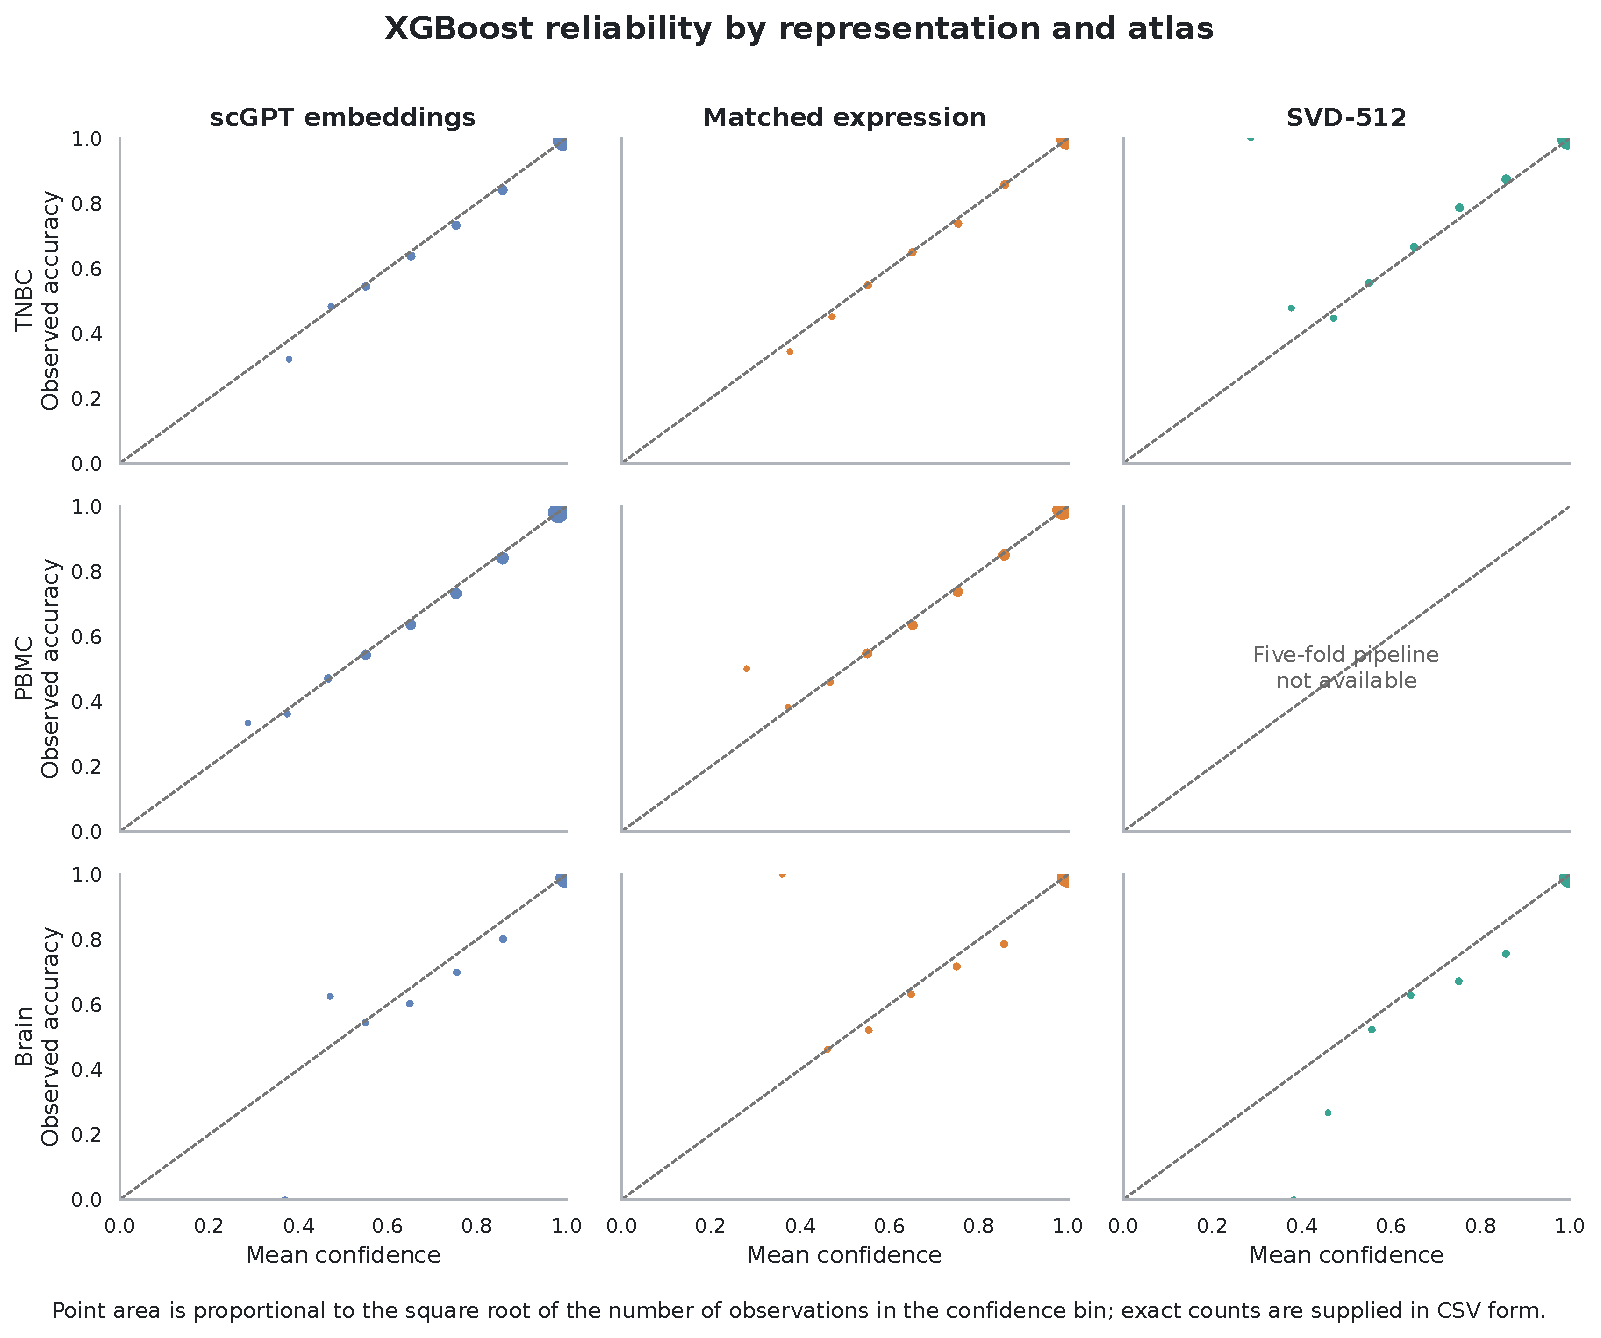
\includegraphics[width=\textwidth]{supplementary_reliability_xgboost.pdf}\caption{Reliability of the final XGBoost pipelines across the human atlases. Point size encodes confidence-bin count; exact bin edges, counts, mean confidence and accuracy are supplied in \texttt{human\_reliability\_bins.csv}.}\label{fig:s-reliability}\end{figure}

\clearpage\section{PBMC biological error profile}

\begin{figure}[H]\centering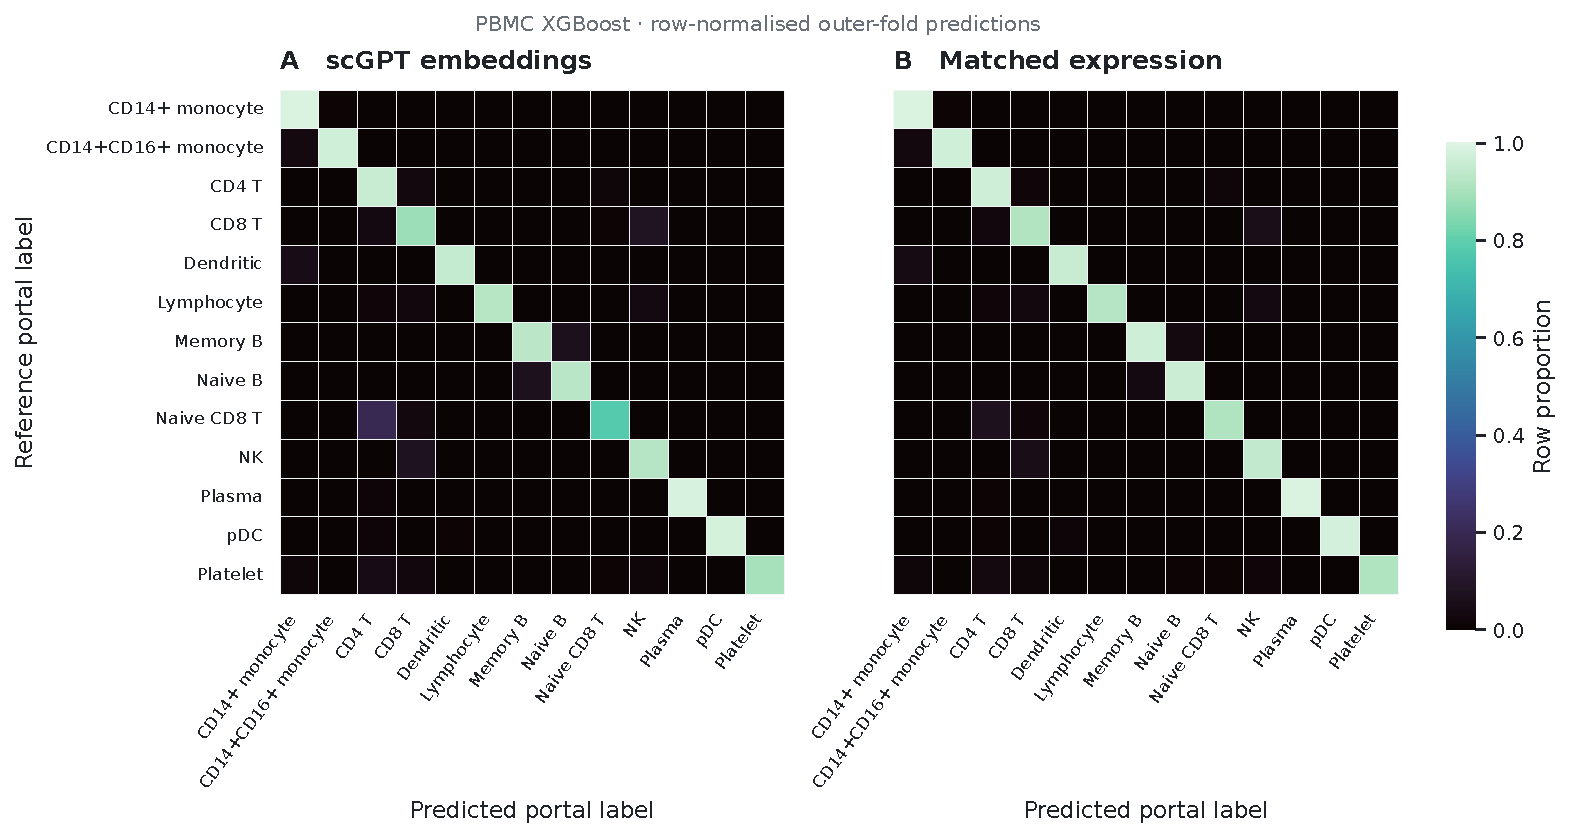
\includegraphics[width=\textwidth]{supplementary_confusion_indonesia_pbmc.pdf}\caption{Row-normalized PBMC confusion matrices for XGBoost. Portal annotations are used as reference labels.}\end{figure}

{\footnotesize\setlength{\tabcolsep}{3pt}
\begin{longtable}{>{\raggedright\arraybackslash}p{4.2cm}llrrrr}
\caption{Complete per-class metrics for PBMC.}\label{tab:s-perclass-pbmc}\\
\toprule
Portal class & Representation & Classifier & Support & Precision & Recall & F1 \\
\midrule
\endfirsthead
\multicolumn{7}{c}{\tablename\ \thetable{} continued}\\
\toprule
Portal class & Representation & Classifier & Support & Precision & Recall & F1 \\
\midrule
\endhead
\midrule
\multicolumn{7}{r}{Continued on next page}\\
\endfoot
\bottomrule
\endlastfoot
CD4-positive, alpha-beta T cell & Matched expression & Logistic regression & 135461 & 0.967 & 0.970 & 0.968 \\
CD8-positive, alpha-beta T cell & Matched expression & Logistic regression & 91629 & 0.922 & 0.920 & 0.921 \\
natural killer cell & Matched expression & Logistic regression & 81409 & 0.939 & 0.944 & 0.942 \\
CD14-positive monocyte & Matched expression & Logistic regression & 51039 & 0.990 & 0.992 & 0.991 \\
memory B cell & Matched expression & Logistic regression & 27172 & 0.968 & 0.968 & 0.968 \\
naive thymus-derived CD8-positive, alpha-beta T cell & Matched expression & Logistic regression & 26375 & 0.920 & 0.901 & 0.910 \\
naive B cell & Matched expression & Logistic regression & 21672 & 0.961 & 0.961 & 0.961 \\
CD14-positive, CD16-positive monocyte & Matched expression & Logistic regression & 13503 & 0.981 & 0.978 & 0.979 \\
dendritic cell, human & Matched expression & Logistic regression & 4374 & 0.967 & 0.965 & 0.966 \\
platelet & Matched expression & Logistic regression & 3013 & 0.929 & 0.924 & 0.926 \\
plasma cell & Matched expression & Logistic regression & 2425 & 0.993 & 0.989 & 0.991 \\
plasmacytoid dendritic cell & Matched expression & Logistic regression & 2005 & 0.994 & 0.986 & 0.990 \\
lymphocyte & Matched expression & Logistic regression & 1957 & 0.967 & 0.943 & 0.955 \\
CD4-positive, alpha-beta T cell & scGPT embeddings & Logistic regression & 135461 & 0.954 & 0.961 & 0.957 \\
CD8-positive, alpha-beta T cell & scGPT embeddings & Logistic regression & 91629 & 0.906 & 0.902 & 0.904 \\
natural killer cell & scGPT embeddings & Logistic regression & 81409 & 0.925 & 0.934 & 0.930 \\
CD14-positive monocyte & scGPT embeddings & Logistic regression & 51039 & 0.988 & 0.990 & 0.989 \\
memory B cell & scGPT embeddings & Logistic regression & 27172 & 0.955 & 0.951 & 0.953 \\
naive thymus-derived CD8-positive, alpha-beta T cell & scGPT embeddings & Logistic regression & 26375 & 0.900 & 0.847 & 0.873 \\
naive B cell & scGPT embeddings & Logistic regression & 21672 & 0.939 & 0.945 & 0.942 \\
CD14-positive, CD16-positive monocyte & scGPT embeddings & Logistic regression & 13503 & 0.976 & 0.974 & 0.975 \\
dendritic cell, human & scGPT embeddings & Logistic regression & 4374 & 0.962 & 0.959 & 0.961 \\
platelet & scGPT embeddings & Logistic regression & 3013 & 0.927 & 0.923 & 0.925 \\
plasma cell & scGPT embeddings & Logistic regression & 2425 & 0.994 & 0.993 & 0.994 \\
plasmacytoid dendritic cell & scGPT embeddings & Logistic regression & 2005 & 0.989 & 0.988 & 0.988 \\
lymphocyte & scGPT embeddings & Logistic regression & 1957 & 0.957 & 0.947 & 0.952 \\
CD4-positive, alpha-beta T cell & SVD-512 & Logistic regression & 135461 & 0.966 & 0.970 & 0.968 \\
CD8-positive, alpha-beta T cell & SVD-512 & Logistic regression & 91629 & 0.919 & 0.916 & 0.918 \\
natural killer cell & SVD-512 & Logistic regression & 81409 & 0.935 & 0.940 & 0.937 \\
CD14-positive monocyte & SVD-512 & Logistic regression & 51039 & 0.990 & 0.991 & 0.990 \\
memory B cell & SVD-512 & Logistic regression & 27172 & 0.968 & 0.968 & 0.968 \\
naive thymus-derived CD8-positive, alpha-beta T cell & SVD-512 & Logistic regression & 26375 & 0.920 & 0.901 & 0.910 \\
naive B cell & SVD-512 & Logistic regression & 21672 & 0.960 & 0.961 & 0.960 \\
CD14-positive, CD16-positive monocyte & SVD-512 & Logistic regression & 13503 & 0.981 & 0.978 & 0.979 \\
dendritic cell, human & SVD-512 & Logistic regression & 4374 & 0.962 & 0.961 & 0.962 \\
platelet & SVD-512 & Logistic regression & 3013 & 0.930 & 0.919 & 0.924 \\
plasma cell & SVD-512 & Logistic regression & 2425 & 0.993 & 0.993 & 0.993 \\
plasmacytoid dendritic cell & SVD-512 & Logistic regression & 2005 & 0.991 & 0.986 & 0.989 \\
lymphocyte & SVD-512 & Logistic regression & 1957 & 0.964 & 0.934 & 0.948 \\
CD4-positive, alpha-beta T cell & Matched expression & Random forest & 135461 & 0.964 & 0.963 & 0.964 \\
CD8-positive, alpha-beta T cell & Matched expression & Random forest & 91629 & 0.902 & 0.904 & 0.903 \\
natural killer cell & Matched expression & Random forest & 81409 & 0.919 & 0.933 & 0.926 \\
CD14-positive monocyte & Matched expression & Random forest & 51039 & 0.981 & 0.990 & 0.986 \\
memory B cell & Matched expression & Random forest & 27172 & 0.953 & 0.949 & 0.951 \\
naive thymus-derived CD8-positive, alpha-beta T cell & Matched expression & Random forest & 26375 & 0.903 & 0.902 & 0.903 \\
naive B cell & Matched expression & Random forest & 21672 & 0.941 & 0.938 & 0.940 \\
CD14-positive, CD16-positive monocyte & Matched expression & Random forest & 13503 & 0.977 & 0.955 & 0.966 \\
dendritic cell, human & Matched expression & Random forest & 4374 & 0.968 & 0.935 & 0.951 \\
platelet & Matched expression & Random forest & 3013 & 0.949 & 0.740 & 0.831 \\
plasma cell & Matched expression & Random forest & 2425 & 0.997 & 0.979 & 0.988 \\
plasmacytoid dendritic cell & Matched expression & Random forest & 2005 & 0.996 & 0.947 & 0.971 \\
lymphocyte & Matched expression & Random forest & 1957 & 0.991 & 0.749 & 0.853 \\
CD4-positive, alpha-beta T cell & scGPT embeddings & Random forest & 135461 & 0.897 & 0.957 & 0.926 \\
CD8-positive, alpha-beta T cell & scGPT embeddings & Random forest & 91629 & 0.868 & 0.857 & 0.862 \\
natural killer cell & scGPT embeddings & Random forest & 81409 & 0.899 & 0.911 & 0.905 \\
CD14-positive monocyte & scGPT embeddings & Random forest & 51039 & 0.982 & 0.990 & 0.986 \\
memory B cell & scGPT embeddings & Random forest & 27172 & 0.923 & 0.919 & 0.921 \\
naive thymus-derived CD8-positive, alpha-beta T cell & scGPT embeddings & Random forest & 26375 & 0.901 & 0.616 & 0.732 \\
naive B cell & scGPT embeddings & Random forest & 21672 & 0.901 & 0.905 & 0.903 \\
CD14-positive, CD16-positive monocyte & scGPT embeddings & Random forest & 13503 & 0.970 & 0.964 & 0.967 \\
dendritic cell, human & scGPT embeddings & Random forest & 4374 & 0.968 & 0.938 & 0.953 \\
platelet & scGPT embeddings & Random forest & 3013 & 0.928 & 0.829 & 0.875 \\
plasma cell & scGPT embeddings & Random forest & 2425 & 0.997 & 0.980 & 0.988 \\
plasmacytoid dendritic cell & scGPT embeddings & Random forest & 2005 & 0.993 & 0.974 & 0.983 \\
lymphocyte & scGPT embeddings & Random forest & 1957 & 0.978 & 0.823 & 0.893 \\
CD4-positive, alpha-beta T cell & Matched expression & XGBoost & 135461 & 0.969 & 0.968 & 0.968 \\
CD8-positive, alpha-beta T cell & Matched expression & XGBoost & 91629 & 0.922 & 0.918 & 0.920 \\
natural killer cell & Matched expression & XGBoost & 81409 & 0.936 & 0.945 & 0.940 \\
CD14-positive monocyte & Matched expression & XGBoost & 51039 & 0.988 & 0.992 & 0.990 \\
memory B cell & Matched expression & XGBoost & 27172 & 0.970 & 0.967 & 0.969 \\
naive thymus-derived CD8-positive, alpha-beta T cell & Matched expression & XGBoost & 26375 & 0.915 & 0.912 & 0.913 \\
naive B cell & Matched expression & XGBoost & 21672 & 0.961 & 0.961 & 0.961 \\
CD14-positive, CD16-positive monocyte & Matched expression & XGBoost & 13503 & 0.981 & 0.972 & 0.976 \\
dendritic cell, human & Matched expression & XGBoost & 4374 & 0.968 & 0.955 & 0.961 \\
platelet & Matched expression & XGBoost & 3013 & 0.924 & 0.914 & 0.919 \\
plasma cell & Matched expression & XGBoost & 2425 & 0.995 & 0.989 & 0.992 \\
plasmacytoid dendritic cell & Matched expression & XGBoost & 2005 & 0.994 & 0.977 & 0.985 \\
lymphocyte & Matched expression & XGBoost & 1957 & 0.973 & 0.921 & 0.946 \\
CD4-positive, alpha-beta T cell & scGPT embeddings & XGBoost & 135461 & 0.936 & 0.955 & 0.945 \\
CD8-positive, alpha-beta T cell & scGPT embeddings & XGBoost & 91629 & 0.884 & 0.880 & 0.882 \\
natural killer cell & scGPT embeddings & XGBoost & 81409 & 0.909 & 0.921 & 0.915 \\
CD14-positive monocyte & scGPT embeddings & XGBoost & 51039 & 0.986 & 0.989 & 0.987 \\
memory B cell & scGPT embeddings & XGBoost & 27172 & 0.941 & 0.933 & 0.937 \\
naive thymus-derived CD8-positive, alpha-beta T cell & scGPT embeddings & XGBoost & 26375 & 0.891 & 0.778 & 0.830 \\
naive B cell & scGPT embeddings & XGBoost & 21672 & 0.918 & 0.927 & 0.923 \\
CD14-positive, CD16-positive monocyte & scGPT embeddings & XGBoost & 13503 & 0.970 & 0.969 & 0.970 \\
dendritic cell, human & scGPT embeddings & XGBoost & 4374 & 0.963 & 0.946 & 0.954 \\
platelet & scGPT embeddings & XGBoost & 3013 & 0.909 & 0.895 & 0.902 \\
plasma cell & scGPT embeddings & XGBoost & 2425 & 0.991 & 0.985 & 0.988 \\
plasmacytoid dendritic cell & scGPT embeddings & XGBoost & 2005 & 0.990 & 0.980 & 0.985 \\
lymphocyte & scGPT embeddings & XGBoost & 1957 & 0.958 & 0.922 & 0.940 \\
\end{longtable}
}

\clearpage\section{Brain biological error profile}

\begin{figure}[H]\centering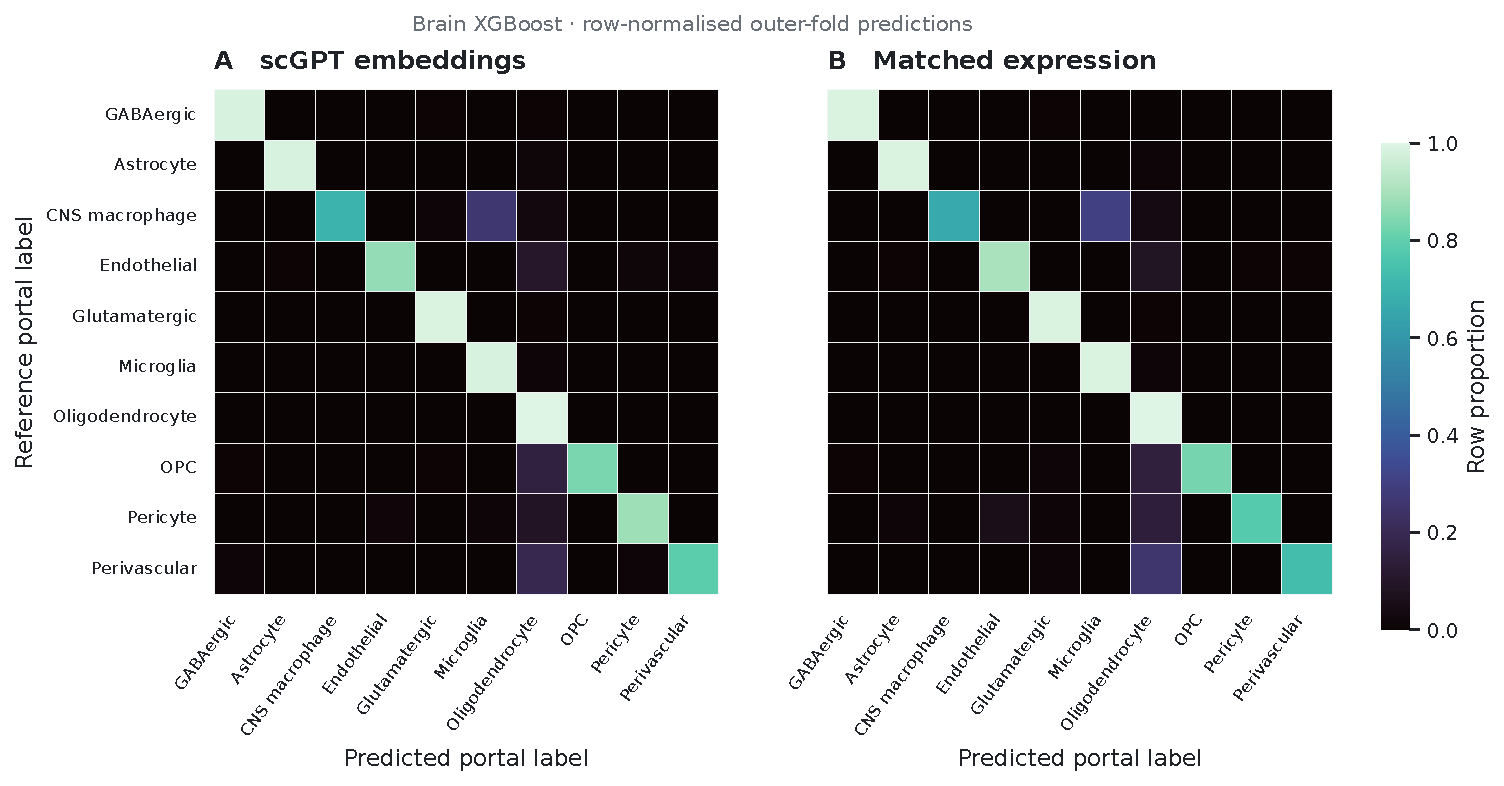
\includegraphics[width=\textwidth]{supplementary_confusion_brain_atlas.pdf}\caption{Row-normalized Brain confusion matrices for XGBoost. Portal annotations are used as reference labels.}\end{figure}

{\footnotesize\setlength{\tabcolsep}{3pt}
\begin{longtable}{>{\raggedright\arraybackslash}p{4.2cm}llrrrr}
\caption{Complete per-class metrics for Brain.}\label{tab:s-perclass-brain}\\
\toprule
Portal class & Representation & Classifier & Support & Precision & Recall & F1 \\
\midrule
\endfirsthead
\multicolumn{7}{c}{\tablename\ \thetable{} continued}\\
\toprule
Portal class & Representation & Classifier & Support & Precision & Recall & F1 \\
\midrule
\endhead
\midrule
\multicolumn{7}{r}{Continued on next page}\\
\endfoot
\bottomrule
\endlastfoot
oligodendrocyte & Matched expression & Logistic regression & 37430 & 0.981 & 0.995 & 0.988 \\
glutamatergic neuron & Matched expression & Logistic regression & 18177 & 0.994 & 0.991 & 0.993 \\
GABAergic neuron & Matched expression & Logistic regression & 8310 & 0.989 & 0.990 & 0.989 \\
astrocyte & Matched expression & Logistic regression & 5042 & 0.995 & 0.990 & 0.993 \\
microglial cell & Matched expression & Logistic regression & 3038 & 0.982 & 0.984 & 0.983 \\
oligodendrocyte precursor cell & Matched expression & Logistic regression & 3014 & 0.950 & 0.833 & 0.888 \\
endothelial cell & Matched expression & Logistic regression & 247 & 0.968 & 0.850 & 0.905 \\
central nervous system macrophage & Matched expression & Logistic regression & 113 & 0.769 & 0.619 & 0.686 \\
perivascular cell & Matched expression & Logistic regression & 105 & 0.987 & 0.714 & 0.829 \\
pericyte & Matched expression & Logistic regression & 104 & 0.976 & 0.769 & 0.860 \\
oligodendrocyte & scGPT embeddings & Logistic regression & 37430 & 0.983 & 0.997 & 0.990 \\
glutamatergic neuron & scGPT embeddings & Logistic regression & 18177 & 0.994 & 0.992 & 0.993 \\
GABAergic neuron & scGPT embeddings & Logistic regression & 8310 & 0.988 & 0.990 & 0.989 \\
astrocyte & scGPT embeddings & Logistic regression & 5042 & 0.993 & 0.990 & 0.991 \\
microglial cell & scGPT embeddings & Logistic regression & 3038 & 0.981 & 0.992 & 0.987 \\
oligodendrocyte precursor cell & scGPT embeddings & Logistic regression & 3014 & 0.976 & 0.829 & 0.897 \\
endothelial cell & scGPT embeddings & Logistic regression & 247 & 0.970 & 0.911 & 0.939 \\
central nervous system macrophage & scGPT embeddings & Logistic regression & 113 & 0.940 & 0.690 & 0.796 \\
perivascular cell & scGPT embeddings & Logistic regression & 105 & 0.947 & 0.848 & 0.894 \\
pericyte & scGPT embeddings & Logistic regression & 104 & 0.931 & 0.913 & 0.922 \\
oligodendrocyte & SVD-512 & Logistic regression & 37430 & 0.981 & 0.996 & 0.988 \\
glutamatergic neuron & SVD-512 & Logistic regression & 18177 & 0.994 & 0.991 & 0.993 \\
GABAergic neuron & SVD-512 & Logistic regression & 8310 & 0.989 & 0.989 & 0.989 \\
astrocyte & SVD-512 & Logistic regression & 5042 & 0.995 & 0.988 & 0.992 \\
microglial cell & SVD-512 & Logistic regression & 3038 & 0.981 & 0.980 & 0.981 \\
oligodendrocyte precursor cell & SVD-512 & Logistic regression & 3014 & 0.954 & 0.833 & 0.890 \\
endothelial cell & SVD-512 & Logistic regression & 247 & 0.963 & 0.834 & 0.894 \\
central nervous system macrophage & SVD-512 & Logistic regression & 113 & 0.704 & 0.611 & 0.654 \\
perivascular cell & SVD-512 & Logistic regression & 105 & 0.986 & 0.695 & 0.816 \\
pericyte & SVD-512 & Logistic regression & 104 & 0.954 & 0.798 & 0.869 \\
oligodendrocyte & Matched expression & Random forest & 37430 & 0.975 & 0.998 & 0.987 \\
glutamatergic neuron & Matched expression & Random forest & 18177 & 0.997 & 0.984 & 0.991 \\
GABAergic neuron & Matched expression & Random forest & 8310 & 0.986 & 0.990 & 0.988 \\
astrocyte & Matched expression & Random forest & 5042 & 0.995 & 0.986 & 0.991 \\
microglial cell & Matched expression & Random forest & 3038 & 0.974 & 0.990 & 0.982 \\
oligodendrocyte precursor cell & Matched expression & Random forest & 3014 & 0.991 & 0.828 & 0.902 \\
endothelial cell & Matched expression & Random forest & 247 & 0.963 & 0.729 & 0.829 \\
central nervous system macrophage & Matched expression & Random forest & 113 & 0.958 & 0.407 & 0.571 \\
perivascular cell & Matched expression & Random forest & 105 & 0.982 & 0.533 & 0.691 \\
pericyte & Matched expression & Random forest & 104 & 0.985 & 0.625 & 0.765 \\
oligodendrocyte & scGPT embeddings & Random forest & 37430 & 0.977 & 0.998 & 0.987 \\
glutamatergic neuron & scGPT embeddings & Random forest & 18177 & 0.994 & 0.989 & 0.991 \\
GABAergic neuron & scGPT embeddings & Random forest & 8310 & 0.991 & 0.980 & 0.985 \\
astrocyte & scGPT embeddings & Random forest & 5042 & 0.994 & 0.986 & 0.990 \\
microglial cell & scGPT embeddings & Random forest & 3038 & 0.982 & 0.989 & 0.986 \\
oligodendrocyte precursor cell & scGPT embeddings & Random forest & 3014 & 0.992 & 0.830 & 0.904 \\
endothelial cell & scGPT embeddings & Random forest & 247 & 0.976 & 0.810 & 0.885 \\
central nervous system macrophage & scGPT embeddings & Random forest & 113 & 0.914 & 0.655 & 0.763 \\
perivascular cell & scGPT embeddings & Random forest & 105 & 0.971 & 0.648 & 0.777 \\
pericyte & scGPT embeddings & Random forest & 104 & 0.973 & 0.702 & 0.816 \\
oligodendrocyte & SVD-512 & Random forest & 37430 & 0.980 & 0.998 & 0.989 \\
glutamatergic neuron & SVD-512 & Random forest & 18177 & 0.995 & 0.991 & 0.993 \\
GABAergic neuron & SVD-512 & Random forest & 8310 & 0.988 & 0.992 & 0.990 \\
astrocyte & SVD-512 & Random forest & 5042 & 0.993 & 0.994 & 0.993 \\
microglial cell & SVD-512 & Random forest & 3038 & 0.964 & 0.990 & 0.977 \\
oligodendrocyte precursor cell & SVD-512 & Random forest & 3014 & 0.998 & 0.835 & 0.909 \\
endothelial cell & SVD-512 & Random forest & 247 & 0.969 & 0.623 & 0.759 \\
central nervous system macrophage & SVD-512 & Random forest & 113 & 0.920 & 0.204 & 0.333 \\
perivascular cell & SVD-512 & Random forest & 105 & 0.971 & 0.629 & 0.763 \\
pericyte & SVD-512 & Random forest & 104 & 0.971 & 0.644 & 0.775 \\
oligodendrocyte & Matched expression & XGBoost & 37430 & 0.981 & 0.998 & 0.990 \\
glutamatergic neuron & Matched expression & XGBoost & 18177 & 0.996 & 0.991 & 0.994 \\
GABAergic neuron & Matched expression & XGBoost & 8310 & 0.989 & 0.992 & 0.990 \\
astrocyte & Matched expression & XGBoost & 5042 & 0.994 & 0.991 & 0.992 \\
microglial cell & Matched expression & XGBoost & 3038 & 0.982 & 0.988 & 0.985 \\
oligodendrocyte precursor cell & Matched expression & XGBoost & 3014 & 0.984 & 0.831 & 0.901 \\
endothelial cell & Matched expression & XGBoost & 247 & 0.970 & 0.903 & 0.935 \\
central nervous system macrophage & Matched expression & XGBoost & 113 & 0.938 & 0.664 & 0.777 \\
perivascular cell & Matched expression & XGBoost & 105 & 0.975 & 0.733 & 0.837 \\
pericyte & Matched expression & XGBoost & 104 & 0.942 & 0.779 & 0.853 \\
oligodendrocyte & scGPT embeddings & XGBoost & 37430 & 0.981 & 0.997 & 0.989 \\
glutamatergic neuron & scGPT embeddings & XGBoost & 18177 & 0.995 & 0.991 & 0.993 \\
GABAergic neuron & scGPT embeddings & XGBoost & 8310 & 0.990 & 0.988 & 0.989 \\
astrocyte & scGPT embeddings & XGBoost & 5042 & 0.994 & 0.988 & 0.991 \\
microglial cell & scGPT embeddings & XGBoost & 3038 & 0.982 & 0.988 & 0.985 \\
oligodendrocyte precursor cell & scGPT embeddings & XGBoost & 3014 & 0.984 & 0.833 & 0.902 \\
endothelial cell & scGPT embeddings & XGBoost & 247 & 0.968 & 0.870 & 0.917 \\
central nervous system macrophage & scGPT embeddings & XGBoost & 113 & 0.868 & 0.699 & 0.775 \\
perivascular cell & scGPT embeddings & XGBoost & 105 & 0.922 & 0.790 & 0.851 \\
pericyte & scGPT embeddings & XGBoost & 104 & 0.939 & 0.885 & 0.911 \\
oligodendrocyte & SVD-512 & XGBoost & 37430 & 0.983 & 0.998 & 0.990 \\
glutamatergic neuron & SVD-512 & XGBoost & 18177 & 0.995 & 0.993 & 0.994 \\
GABAergic neuron & SVD-512 & XGBoost & 8310 & 0.989 & 0.992 & 0.990 \\
astrocyte & SVD-512 & XGBoost & 5042 & 0.995 & 0.992 & 0.993 \\
microglial cell & SVD-512 & XGBoost & 3038 & 0.975 & 0.994 & 0.984 \\
oligodendrocyte precursor cell & SVD-512 & XGBoost & 3014 & 0.986 & 0.836 & 0.905 \\
endothelial cell & SVD-512 & XGBoost & 247 & 0.970 & 0.789 & 0.871 \\
central nervous system macrophage & SVD-512 & XGBoost & 113 & 0.921 & 0.513 & 0.659 \\
perivascular cell & SVD-512 & XGBoost & 105 & 0.945 & 0.657 & 0.775 \\
pericyte & SVD-512 & XGBoost & 104 & 0.976 & 0.798 & 0.878 \\
\end{longtable}
}

\clearpage\section{Pig-pancreas cross-species stress test}

The porcine object contained one donor ID; this analysis therefore uses a random cell split and is excluded from the human primary summary. The whole-human checkpoint was applied by exact/uppercase gene-symbol matching without an orthology map. Results should be read only as a stress test.

{\footnotesize\setlength{\tabcolsep}{3pt}
\begin{longtable}{llrrrrrrr}
\caption{Pig-pancreas stress-test metrics.}\label{tab:s-pig}\\
\toprule
Representation & Classifier & Train & Test & Macro F1 & Accuracy & ECE & Brier & NLL \\
\midrule
\endfirsthead
\multicolumn{9}{c}{\tablename\ \thetable{} continued}\\
\toprule
Representation & Classifier & Train & Test & Macro F1 & Accuracy & ECE & Brier & NLL \\
\midrule
\endhead
\midrule
\multicolumn{9}{r}{Continued on next page}\\
\endfoot
\bottomrule
\endlastfoot
Matched expression & Logistic regression & 17644 & 4412 & 0.988 & 0.997 & 0.002 & 0.005 & 0.012 \\
scGPT embeddings & Logistic regression & 17644 & 4412 & 0.966 & 0.993 & 0.002 & 0.011 & 0.024 \\
SVD-512 & Logistic regression & 17644 & 4412 & 0.987 & 0.997 & 0.003 & 0.004 & 0.008 \\
Matched expression & Random forest & 17644 & 4412 & 0.989 & 0.995 & 0.005 & 0.008 & 0.017 \\
scGPT embeddings & Random forest & 17644 & 4412 & 0.613 & 0.943 & 0.049 & 0.090 & 0.183 \\
SVD-512 & Random forest & 17644 & 4412 & 0.938 & 0.995 & 0.011 & 0.010 & 0.025 \\
Matched expression & XGBoost & 17644 & 4412 & 0.992 & 0.997 & 0.002 & 0.006 & 0.011 \\
scGPT embeddings & XGBoost & 17644 & 4412 & 0.888 & 0.974 & 0.011 & 0.040 & 0.084 \\
SVD-512 & XGBoost & 17644 & 4412 & 0.967 & 0.996 & 0.002 & 0.006 & 0.012 \\
\end{longtable}
}

\clearpage\section{Machine-readable audit material}

The reproducibility archive contains the complete confusion matrices, reliability-bin counts, strict-scarcity seed-level results, selected genes for every outer fold, SVD explained-variance audits, retained hyperparameter traces, model timings, software versions, checkpoint hashes and the original-index alignment records used to verify the out-of-fold partition. The pipeline-coverage table identifies every representation--classifier combination admitted to aggregation.


\end{document}
